\documentclass[12pt,letterpaper]{exam}
\usepackage[lmargin=1in,rmargin=1in,tmargin=1in,bmargin=1in]{geometry}
\usepackage{../style/exams}

% -------------------
% Course & Exam Information
% -------------------
\newcommand{\course}{MAT 108: Exam 2}
\renewcommand{\term}{Fall -- 2022}
\newcommand{\examdate}{11/10/2022}
\newcommand{\timelimit}{85 Minutes}

\setbool{hideans}{false} % Student: True; Instructor: False

% -------------------
% Content
% -------------------
\begin{document}

\examtitle
\instructions{Write your name on the appropriate line on the exam cover sheet. This exam contains \numpages\ pages (including this cover page) and \numquestions\ questions. Check that you have every page of the exam. Answer the questions in the spaces provided on the question sheets. Be sure to answer every part of each question and show all your work. If you run out of room for an answer, continue on the back of the page --- being sure to indicate the problem number.} 
\scores
\bottomline
\newpage

% ---------
% Questions
% ---------
\begin{questions}

% Question 1
\newpage
\question[15] Researchers studying changing viewpoints for youths in education took a survey of 1,001 students in middle school. The researchers asked the students what they believed was the most useful thing in school: having high grades, being popular, or athletic ability. The results, broken down by type of school, are found below. \par
	\begin{table}[!ht]
	\centering
	\begin{tabular}{| l || c | c | c || c |} \hline 
	& Public & Private & Charter & Total \\ \hline \hline
	Grades & 87 & 115 & 82 & 284 \\ \hline
	Popularity & 165 & 91 & 177 & 433 \\ \hline
	Athleticism & 102 & 88 & 94 & 284 \\ \hline \hline
	Total & 354 & 294 & 353 & 1001 \\ \hline
	\end{tabular}
	\end{table} \par
Assuming that this survey is representative of public, private, and charter schools as a whole, determine\dots

\begin{enumerate}[(a)]
\item \dots the percentage of students that attend private schools. 
\item \dots the percentage of students that believe grades are the most useful thing. 
\item \dots the percentage of students that are in charter schools and believe popularity is the most useful thing. 
\item \dots the percentage of students in public schools that believe athleticism is the most useful thing. 
\item \dots the percentage of students in public school, private school, or believe that athleticism is the most important thing. 
\end{enumerate} \pspace

\sol 
\begin{enumerate}[(a)]
\item \dots the percentage of students that attend private schools. \pvspace{0.3cm}
	\[
	P(\text{private})= \dfrac{294}{1001} \approx 0.2937 \squiggle 29.37\%
	\] \pvspace{0.3cm}

\item \dots the percentage of students that believe grades are the most useful thing. \pvspace{0.3cm}
	\[
	P(\text{grades})= \dfrac{284}{1001} \approx 0.2837 \squiggle 28.37\%
	\] \pvspace{0.3cm}

\item \dots the percentage of students that are in charter schools and believe popularity is the most useful thing. \pvspace{0.3cm}
	\[
	P(\text{charter and popularity})= \dfrac{177}{1001} \approx 0.1768 \squiggle 17.68\%
	\] \pvspace{0.3cm}

\item \dots the percentage of students in public schools that believe athleticism is the most useful thing. \pvspace{0.3cm}
	\[
	P(\text{athleticism} \;|\; \text{public})= \dfrac{102}{354} \approx 0.2881 \squiggle 28.81
	\] \pvspace{0.3cm}

\item \dots the percentage of students in public school, private school, or believe that athleticism is the most important thing. \pvspace{0.3cm}
	\[
	\hspace{-1.2cm} P(\text{public or private or athleticism})= \dfrac{354 + 294 + 284 - 102 - 88}{1001}= \dfrac{742}{1001} \approx 0.7413 \squiggle 74.13\%
	\]
\end{enumerate}



% Question 2
\newpage
\question[10] Several medical researchers believe that `genetic drift' is causing the average cholesterol levels in adults to increase. Hence, previously used thresholds of `high cholesterol' may be too low. The researchers measured the cholesterol levels of 265~individuals and found a sample average of 194.1~mg/dL. If cholesterol levels in adults have a standard deviation of 3.8~mg/dL, construct a 92\% confidence interval for the average cholesterol level in adults. \pvspace{1.5cm}

{\itshape Because the sample size of 265~individuals is sufficiently large, we know that the Central Limit Theorem applies. The underlying population standard deviation is $\sigma= 3.8$~mg/dL. We have a sample average of $\overline{x}= 194.1$~mg/dL on a sample size of $n= 265$~individuals. We require a $z$-score that corresponds to $92\% + \frac{100\% - 92\%}{2}= 92\% + 4\%= 96\%$. But then we have $z^* \approx 1.75$. But then we have\dots
	\[
	\begin{aligned}
	\overline{x} \qquad&\pm\qquad z^* \dfrac{\sigma}{\sqrt{n}} \\[0.3cm]
	194.1 \text{ mg/dL} \qquad&\pm\qquad 1.75 \cdot \dfrac{3.8 \text{ mg/dL}}{\sqrt{265}} \\[0.3cm]
	194.1 \text{ mg/dL} \qquad&\pm\qquad 1.75 \cdot 0.233 \text{ mg/dL} \\[0.3cm]
	194.1 \text{ mg/dL} \qquad&\pm\qquad 0.408 \text{ mg/dL} 
	\end{aligned}
	\] \pspace
Note that $194.1 \text{ mg/dL} - 0.408 \text{ mg/dL} \approx 193.7 \text{ mg/dL}$ and $194.1 \text{ mg/dL} + 0.408 \text{ mg/dL} \approx 194.5 \text{ mg/dL}$. \pspace

Therefore, we are 92\% confident that the average adult blood pressure is between 193.7~mg/dL and 194.5~mg/dL. 
}



% Question 3
\newpage
\question[10] Mike is playing a D\&D game with a ten-sided die. He comes across a demogorgon---\#FearTheDemogorgon. Unfortunately, the demogorgon has cloned itself, creating 12~copies. Mike needs to roll a 10 to defeat any single demogorgon. 
	\begin{enumerate}[(a)]
	\item Find the probability that Mike defeats exactly two demogorgons.
	\item Find the probability that Mike defeats four or more demogorgons.
	\item Find the probability that Mike defeats all the demogorgons.
	\item Find the probability that Mike defeats at least one of the demogorgons. 
	\end{enumerate} \pspace

\sol {\itshape Because each dice roll is independent, each roll is either a `success' or `failure' (rolling a 10 or not), there is a fixed number of rolls (12 rolls), and the probability of success is fixed ($p= \frac{1}{10}$), this is a binomial distribution, namely $B \big(12, \frac{1}{10} \big)$.
\begin{enumerate}[(a)]
\item 
	\[
	P(X= 2)= 0.2301
	\] \pspace

\item 
	\[
	\begin{aligned}
	P(X \geq 4)&= P(X= 4) + P(X= 5) + \cdots + P(X= 11) + P(X= 12) \\[0.3cm]
	&\approx 0.0213 + 0.0038 + 0.0005 + 0.0000 + \cdots + 0.0000 \\[0.3cm]
	&= 0.0256
	\end{aligned}
	\] \pspace

\item 
	\[
	P(X= 12) \approx 0.0000
	\] \pspace

\item 
	\[
	P(X \geq 1)= 1 - P(X= 0) \approx 1 - 0.2824= 0.7176
	\]
\end{enumerate}
}



% Question 4
\newpage
\question[15] Students in a class on quantitative methods in business and social science are studying for an exam. If a student studies, there is an 80\% chance that they will pass the exam. If a student does not study, there is a 75\% chance that they will fail the exam. After a brief survey, the instructors estimates that only 60\% of the students will study for the exam. 
	\begin{enumerate}[(a)]
	\item Find the percentage of the students that will study for the exam and pass.
	\item Find the percentage of students that will fail the exam. 
	\item Find the percentage of students that will pass the exam. 
	\item Find the percentage of students that either did not study or will fail the exam.
	\item What percentage of students that did not study will pass the exam anyway?
	\end{enumerate} \pspace

\sol 
\begin{enumerate}[(a)]
\item 
	\[
	P(\text{study and pass})= 0.48
	\] \pspace

\item 
	\[
	P(\text{fail})= 0.12 + 0.30= 0.42
	\] \pspace

\item 
	\[
	P(\text{pass})= 0.48 + 0.10= 0.58
	\] \pspace

\item 
	\[
	P(\text{not study or fail})= 0.10 + 0.30 + 0.12= 0.52
	\] \pspace

\item 
	\[
	P(\text{pass} \;|\; \text{not study})= \dfrac{0.10}{0.10 + 0.30}= \dfrac{0.10}{0.40}= 0.25
	\]
\end{enumerate} \vfill

		\[
		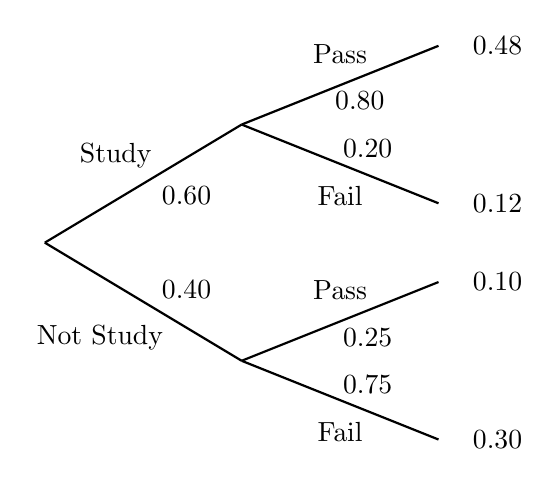
\begin{tikzpicture}[scale= 1.0]
		\def\FirstUpLabel{Study}
		\def\FirstDownLabel{Not Study}
		\def\SecondUpLabel{Pass}
		\def\SecondDownLabel{Fail}
		\def\Up{$0.60$}
		\def\Down{$0.40$}
		\def\UpUp{$0.80$}
		\def\UpDown{$0.20$}
		\def\DownUp{$0.25$}
		\def\DownDown{$0.75$}
		\def\first{$0.48$}
		\def\second{$0.12$}
		\def\third{$0.10$}
		\def\fourth{$0.30$}
		
		\node at (0.9,1.1) {\FirstUpLabel};	
		\node at (0.7,-1.2) {\FirstDownLabel};	
		\node at (1.8,0.6) {\Up};
		\node at (1.8,-0.6) {\Down};
		\draw[thick] (0,0) -- (2.5,1.5);
		\draw[thick] (0,0) -- (2.5,-1.5);
		
		\node at (3.75,2.4) {\SecondUpLabel};
		\node at (3.75,0.6) {\SecondDownLabel};
		\node at (4,1.8) {\UpUp};
		\node at (4.1,1.2) {\UpDown};
		\node at (5.75,2.5) {\first};
		\node at (5.75,0.5) {\second};
		\draw[thick] (2.5,1.5) -- (5,2.5);
		\draw[thick] (2.5,1.5) -- (5,0.5);

		\node at (3.75,-0.6) {\SecondUpLabel};
		\node at (3.75,-2.4) {\SecondDownLabel};
		\node at (4.1,-1.2) {\DownUp};
		\node at (4.1,-1.8) {\DownDown};
		\node at (5.75,-0.5) {\third};	
		\node at (5.75,-2.5) {\fourth};	
		\draw[thick] (2.5,-1.5) -- (5,-0.5);
		\draw[thick] (2.5,-1.5) -- (5,-2.5);
		\end{tikzpicture}
		\]



% Question 5
\newpage
\question[10] Students in a class on quantitative methods in business and social science have just taken an exam. The exam scores were normally distributed with a mean of 45 and standard deviation 11.3. 
	\begin{enumerate}[(a)]
	\item Find the percentage of students that scored at least 65 on the exam. 
	\item Find the minimal score one would need to be in the top 10\% of exam scores. 
	\end{enumerate} \pspace


\sol 
{\itshape 
\begin{enumerate}[(a)]
\item We have\dots
	\[
	z_{65}= \dfrac{65 - 45}{11.3}= \dfrac{20}{11.3} \approx 1.77 \squiggle 0.9616
	\]
But because we want $X \geq 65$, we have $1 - 0.9616= 0.0384$. Therefore, 3.84\% of students scored at least a 65 on the exam. \pspace

\item If you received a score, say $x$, to be in the top 10\%, then 90\% of students would have scored less than you. But then $z_x \squiggle 0.90$. Therefore, we know that $z_x \approx 1.28$. Then we have\dots
	\[
	\begin{aligned}
	z_x&= 1.28 \\[0.3cm]
	\dfrac{x - \mu}{\sigma}&= 1.28 \\[0.3cm]
	\dfrac{x - 45}{11.3}&= 1.28 \\[0.3cm]
	x - 45&= 14.464 \\[0.3cm]
	x&= 59.464
	\end{aligned}
	\]
Therefore, a score of at least approximately 59.5 would put you in the top 10\% of exam scores. 
\end{enumerate}
}



% Question 6
\newpage
\question[10] Local government officials are trying to determine how to allocate public health funds from a recent grant. It is known that approximately 26\% of adults in the US have some type of disability. One of the villages in the county has a population of 2,500 adults.
	\begin{enumerate}[(a)]
	\item What is the probability that less than 620 of these adults will have a disability?
	\item What is the probability that less than 720 of these adults will have a disability?
	\item What is the probability that between 620 and 720 of these adults will have a disability?
	\end{enumerate} \pspace

\sol Suppose that the sample is a simple random sample and that each selection for the sample is independent from the next. Because we have a fixed population of 2,500~adults, each person selected is a `success' or not (has a disability or not), and the chance of `success' is fixed with probability 0.26, this is binomial, namely $B(2500, 0.26)$. Because $np= 2500(0.26)= 650 \geq 10$ and $n(1 - p)= 2500(1 - 0.26)= 2500(0.74)= 1850 \geq 10$, we can approximate this binomial distribution with a normal distribution: $B(n, p) \approx N(np, \sqrt{np(1 - p)})$. Therefore, this distribution is approximately $N(2500(0.26), \sqrt{2500(0.26)(1 - 0.26)}) \approx N(650, 21.9317)$. 

\begin{enumerate}[(a)]
\item We have\dots
	\[
	z_{620}= \dfrac{620 - 650}{21.9317}= \dfrac{-30}{21.9317} \approx -1.37 \squiggle 0.0853
	\]
Therefore, $P(X \leq 620) \approx 0.0853$. \pspace

\item We have\dots
	\[
	z_{720}= \dfrac{720 - 650}{21.9317}= \dfrac{70}{21.9317} \approx 3.19 \squiggle 0.9993
	\]
Therefore, $P(X \leq 720) \approx 0.9993$. \pspace

\item Using (a) and (b), we know that\dots
	\[
	P(620 \leq X \leq 720)= P(X \leq 720) - P(X \leq 620) \approx 0.9993 - 0.0853= 0.9140
	\]
\end{enumerate}



% Question 7
\newpage
\question[10] A researcher is collecting data on sleep and academic performance. They collect data on student's GPA, $g$, and plot it against the average number of hours of sleep, $h$, students had during a given week. They find a linear regression model of $\widehat{g}= 0.028h + 3.5$. A scatterplot of their data with the model is found below.
	\begin{figure}[!ht]
	\centering
	\includegraphics[width=0.48\textwidth]{regplot.png}
	\end{figure}

\begin{enumerate}[(a)]
\item Find the model's prediction of a student's GPA if they slept 8~hours a night.
\item If a student that slept 8~hours a night had a GPA of 3.528, find the residual for this model's prediction of this datapoint. 
\item If the researchers had an $R^2$ value of 0.407263, does this imply a `good' model, i.e. a strong correlation? Explain.
\item Is (c) supported by the scatterplot above? Explain.
\end{enumerate} \pspace

\sol 
{\itshape
\begin{enumerate}[(a)]
\item We have
	\[
	\widehat{y}(8)= 0.028(8) + 3.5= 0.224 + 3.5= 3.724
	\] \pspace
Therefore, the model predicts that a student that sleeps 8~hours a night will have a GPA of 3.724. \pspace

\item We have\dots
	\[
	e_i= y - \widehat{y}= 3.528 - 3.724= -0.196
	\]

\item This is not a `good' model. The $R^2$ value essentially tells you the `percent linearity' of the data. Specifically, $R^2= 0.407263$ implies that approximately 40.7\% of the variation in the data is explained by this linear model. The closer $R^2$ is to 1, the better the explanatory power of the model. Typically, we want $R^2$ to be at least 0.60. Therefore, this $R^2$ value demonstrates a weak predictive power for the model. \pspace

\item Yes. Observe that the line does not `tightly fit' the data. Hence, we expect a rather low value for $R^2$. The larger the $R^2$-value, the `closer' the points are to the linear model. 
\end{enumerate}
}



% Question 8
\newpage
\question[10] A company claims that their warehouse workers are paid more than the national average of \$23.75 per hour. A local journalist doubts the company's claim and surveys 15 of the workers at the warehouse about their hourly wage. The journalist assume that wages at the warehouse have the same standard deviation of \$1.27 as wages nationally for this type of job.
	\begin{enumerate}[(a)]
	\item Find the probability that the average salary of these workers is less than \$23 per hour.
	\item What assumption(s) about the workers' salary do your calculations in (a) require, if any. 
	\end{enumerate} \pspace

\sol 
{\itshape Assuming that the central limit theorem applies, i.e. that the underlying distribution of incomes at this warehouse is normally distributed or that the sample size is sufficiently large ($\geq \approx 30$), then we know that the distribution of sample means of size 15 is approximately distributed as $N(\mu, \sigma/\sqrt{n})$. If we assume that $\mu= 23.75$ and $\sigma= 1.27$, because we have $n= 15$, we have $N(\mu, \sigma/\sqrt{n})= N(23.75, 1.27/\sqrt{15}) \approx N(23.75, 0.328)$. 
\begin{enumerate}[(a)]
\item From the comments above, we have\dots
	\[
	z_{23}= \dfrac{23 - 23.75}{0.328}= \dfrac{-0.75}{0.328} \approx -2.29 \squiggle 0.0110
	\]
Therefore, we have $P(\overline{X} \leq 23)= 0.0110$. \pspace

\item As commented above, the above calculation relies on the fact that the distribution of average incomes of sample of size 15 have distribution $N(23.75, 0.328)$. This required that the central limit theorem applies; that is, this would require either the underlying distribution of warehouse incomes was normally distributed or a sufficiently large sample size. Because the sample size is not sufficiently large, we must assume that the underlying distribution of incomes at this warehouse is normally distributed. 
\end{enumerate}
}



% Question 9
\newpage
\question[10] Read the following two scenarios:
	\begin{enumerate}
	\item[I.] A politician is making claims about immigrants into their country. They cite data showing that $68.3\%$ of these immigrants do not have higher education. Because studies have shown that $4.12\%$ of those without higher education will commit violent crimes, they claim that $68.3 \cdot 4.12 \approx 2.81\%$ of these immigrants will commit a violent crime. They also claim that because there were $10,000$ new immigrants last month, there are now $10,\!000 \cdot 0.0281 \approx 281$ new violent criminals in the area.
	\item[II.] Efficiency managers have been hired at a local law firm to improve `work flow' at their company. The efficiency managers gather data and find that $40\%$ of workers handle some type of paperwork while $33\%$ of workers handle some type of data entry. They conclude that at least $40\% + 33\%= 73\%$ of workers at the company either handle some type of paperwork or some type of data entry. 
	\end{enumerate}
Now respond to the following two questions:

\begin{enumerate}[(a)]
\item Is the mathematical claim the politician made in (I) correctly reasoned? Explain.
\item Is the mathematical claim the efficiency managers made in (II) correctly reasoned? Explain.
\end{enumerate} \pspace

\sol 
{\itshape
\begin{enumerate}[(a)]
\item The politician's claim is not correctly reasoned. They are assuming that these events are independent. One can only multiply probabilities if the events are independent. For instance, it might be that there is a much lower chance an immigrant without higher education will commit a crime, perhaps for fear of deportation. [In fact, studies suggest this is the case.] There may also be arguments to suggest that they are more likely to commit a violent crime. Regardless, these events are, in principle, very dependent. Therefore, one cannot simply multiply these probabilities. \pspace

\item The efficiency manager's claim is not correctly reasoned. To add percentages/probabilities, one need know that the underlying events are disjoint. Otherwise, one would overestimate the percentage/probability. In principle, there may be workers at this firm that both handle paperwork and data entry, in which case they would be overestimating the percentage of workers at this company that perform either task. [In fact, this is very likely to be the case.] Therefore, one cannot simply add these percentages. 
\end{enumerate}
}


\end{questions}
\end{document}